\documentclass[border=2pt]{standalone}
\usepackage{tikz}
\usetikzlibrary{shapes, arrows.meta, decorations.pathreplacing, positioning}

\begin{document}

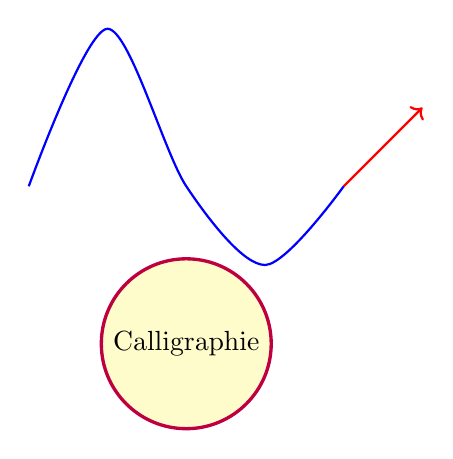
\begin{tikzpicture}
    % Courbe élégante avec un trait doux
    \draw[thick, smooth, blue] plot coordinates {(0,0) (1,2) (2,0) (3,-1) (4,0)};
    
    % Ajout d'une flèche avec décoration
    \draw[thick,->,red] (4,0) -- (5,1);
    
    % Créer un cercle calligraphique
    \node[circle, draw=purple, fill=yellow!20, very thick, text centered] at (2, -2) {Calligraphie};
\end{tikzpicture}

\end{document}
